\documentclass{article}
\usepackage{flafter}
\usepackage{amsmath}
\usepackage{booktabs}
\usepackage{graphicx}
\usepackage{hyperref}
\usepackage{listings}
\usepackage[section]{placeins}
\usepackage{subcaption}

\begin{document}

\title{SaltNet: Resource-Efficient Deep Learning Approach for Grayscale Image Denoising} % Example Title -  You should refine this

\author{Mostafa Kamal \\ \href{mailto:mos.kamal@nu.edu.eg}{mos.kamal@nu.edu.eg} }

\date{\today}

\maketitle


\begin{abstract}
    Image denoising is a crucial preprocessing step in various computer vision applications, yet remains challenging due to the diverse nature of noise and the trade-off between denoising efficacy and computational cost.  This paper introduces SaltNet, a multi-pathway, resource-efficient deep learning network for grayscale image denoising, designed to handle a range of noise types including Bernoulli, Poisson, Salt and Pepper, and Gaussian noise. SaltNet architecture integrates parallel pathways of Selective Convolutional (SeConv) blocks, adept denoising salt and pepper corrupted images\cite{Rafiee2021}, and novel Anisotropic Diffusion blocks, designed to smooth images while preserving structural details.  The features extracted from these pathways are fused and further refined by a shallow Transformer network, inspired by Restormer\cite{Zamir2022}, to capture long-range dependencies. Finally, an AutoEncoder, U-Net structure with skip connections, module serves as a post-processing stage to enhance perceptual quality\cite{Wu2022}.  Experimental results demonstrate that SaltNet achieves denoising performance competitive with state-of-the-art methods like Restormer, while exhibiting efficient resource utilization in terms of both runtime and memory consumption.

\end{abstract}

\section{Literature Review}
\label{sec:literature_review}
    
Traditional image denoising methods often rely on handcrafted filters or optimization algorithms, which may not generalize well to different noise types. Deep learning-based approaches have proven to be powerful tools for image denoising, achieving state-of-the-art performance on a variety of noise types.

One of the pioneering works in deep learning-based image denoising is DnCNN\cite{Zhang2017}, a deep convolutional neural network designed to remove Gaussian noise. DnCNN demonstrates the ability to handle blind Gaussian denoising, where the noise level is unknown, and can be extended to other image restoration tasks such as super-resolution. Other CNN-based methods have been proposed, including FFDNet\cite{Zhang2018}, which achieves fast and flexible denoising by incorporating noise level information into the network.

While CNNs excel at capturing local dependencies in images, they often struggle to model global image context, which can be crucial for high-quality image restoration. To address this limitation, Transformers, originally developed for natural language processing, have been adapted for image restoration tasks. Transformers utilize self-attention mechanisms to capture global dependencies between pixels, enabling them to effectively learn image priors and achieve impressive results on various restoration tasks.

One notable example is Restormer\cite{Zamir2022}, an efficient Transformer model designed for high-resolution image restoration. Restormer incorporates several key designs in its building blocks, such as multi-head attention and feed-forward networks, to capture long-range pixel dependencies while remaining computationally feasible for large images. Restormer has achieved state-of-the-art performance on various image restoration tasks, including deraining, deblurring, and denoising.

In addition to Gaussian noise, impulse noise, such as salt-and-pepper noise, is another common type of noise that can severely degrade image quality. Traditional methods for salt-and-pepper noise removal often involve median-based filters or adaptive approaches that exploit local image statistics\cite{Memis2021}. Deep learning methods have also been explored for salt-and-pepper noise removal. SeConvNet introduces a new selective convolutional (SeConv) block that effectively restores salt-and-pepper noise corruption in both grayscale and color images, outperforming traditional methods at high noise densities.\cite{Rafiee2021}

An important architecture in deep learning for image processing is the U-Net. This encoder-decoder architecture with skip connections has proven highly effective for tasks that require precise localization, such as segmentation and image-to-image translation. The U-Net's ability to preserve fine details while capturing global context makes it well-suited for image restoration tasks.\cite{Wu2022}

The proposed SaltNet model builds upon the strengths of existing deep learning approaches for image denoising. It incorporates SeConv blocks from SeConvNet to effectively handle salt-and-pepper noise, while also introducing novel anisotropic diffusion blocks to further enhance denoising capabilities. Additionally, SaltNet leverages Transformer blocks, similar to Restormer, to capture long-range dependencies. SaltNet is terminated by an AutoEncoder U-Net-like architecture to enhance ability to capture fine details and long-range pixel dependencies. By combining these different components, SaltNet aims to achieve competitive denoising performance while maintaining resource efficiency.

\section{SaltNet Architecture}
\label{sec:saltnet_architecture}
    The SaltNet architecture is designed with a multi-pathway approach to effectively denoise images while maintaining computational efficiency. As depicted in Figure \ref{fig:saltnet_architecture}, the network ingests a grayscale noisy image and processes it through several parallel pathways before converging to produce the final denoised output. This structure allows SaltNet to leverage different denoising strategies, addressing various noise types effectively.

\begin{figure}[h]
    \centering
    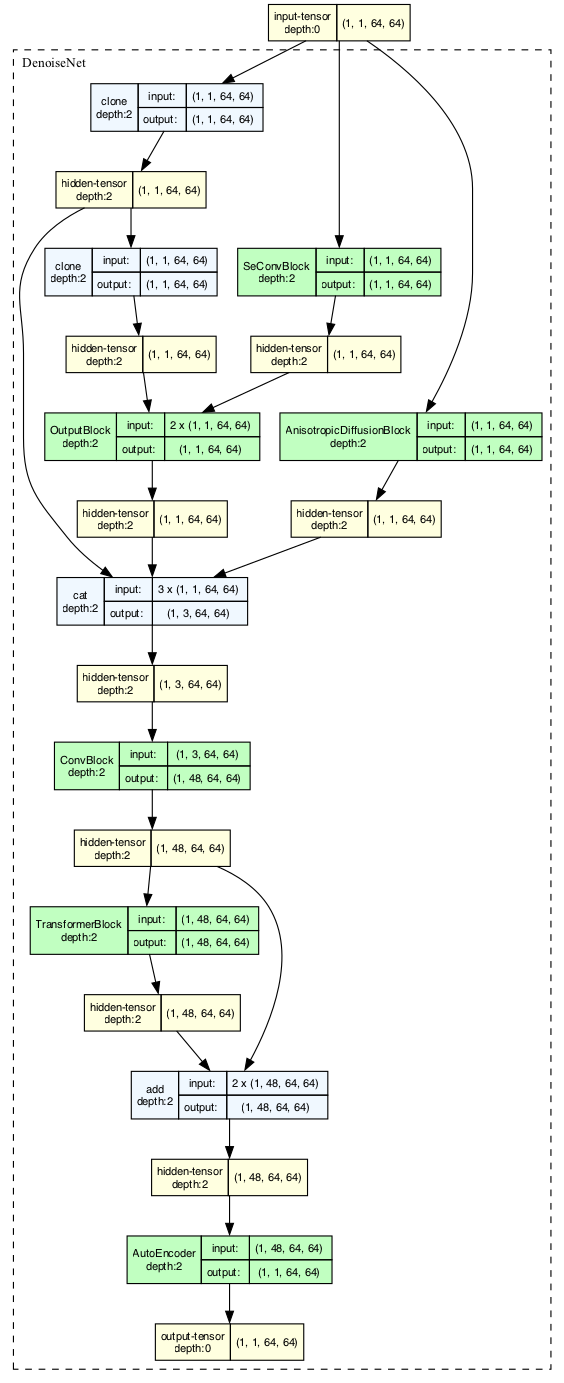
\includegraphics[width=0.8\textwidth]{assets/network_architecture.png}
    \caption{SaltNet Architecture Diagram}
    \label{fig:saltnet_architecture}
\end{figure}

The input noisy image, represented as a tensor of dimensions \( (1, 1, InputHeight, InputWidth) \), is initially cloned and fed into two distinct branches: a stack of Selective Convolutional (SeConv) blocks and a stack of novel Anisotropic Diffusion blocks.

The first branch utilizes \textbf{SeConv blocks}, inspired by the SeConvNet architecture\cite{Rafiee2021}, to effectively address salt-and-pepper noise. We employ a stack of \texttt{7} SeConv blocks, each with increasing kernel sizes to capture multi-scale features. The output of the SeConv block stack is passed through a single \texttt{OutputBlock}: a Conv2d layer, batch normalization layer and ReLU activation, as opposed to a deep CNN network  in the original SeConvNet architecture.

Concurrently, the input image is also processed by a novel stack of \textbf{Anisotropic Diffusion blocks}. This branch uses a novel block implementation, drawing inspiration from anisotropic diffusion filtering but implemented within a deep learning framework. We stack \texttt{5} of these blocks, each applying a learned anisotropic diffusion process to smooth noise while preserving edges and image structures. This component is particularly effective in handling probalistic noise types, such as Gaussian and Poisson noise.

The outputs from both the SeConv and Anisotropic Diffusion branches, along with a cloned version of the original noisy input, are then concatenated along the channel dimension. This concatenated tensor, now with \texttt{3} input channels, is passed into a \textbf{Convolutional Embedding Layer} (\texttt{ConvBlock}). This layer, consisting of a convolutional layer, batch normalization, and ReLU activation, serves to create a feature embedding space with \texttt{48} channels, effectively fusing information from the different denoising pathways.

The resulting feature embeddings are then processed by a small number of \textbf{Transformer blocks}, specifically \texttt{10} blocks. Inspired by the Restormer architecture\cite{Zamir2022}, these transformer blocks leverage multi-head attention mechanisms to capture long-range dependencies within the image. This allows the network to model global image context. To maintain computational efficiency, we limit the number of transformer blocks, compared to deeper Restormer architecture.

Finally, the output of the transformer blocks is fed into an \textbf{AutoEncoder} module. This module inspired by U-Net with skip connections\cite{Wu2022} acts as a post-processing refinement stage. The AutoEncoder, with a depth of \texttt{5}, further refines the denoised features and projects them back to the single-channel grayscale image space. It takes in an input of 48 channel dimensions and produces the final denoised output tensor of dimensions \( (1, 1, InputHeight, InputWidth) \).

By combining these components, SaltNet achieves a robust and efficient denoising architecture. The parallel processing branches allow for specialized handling of different noise characteristics, while the Transformer blocks and AutoEncoder ensure high quality in the final denoised images. This multi-pathway approach, positions SaltNet as a competitive and efficient alternative to existing state-of-the-art denoising networks like Restormer.


\section{Training Details}
\label{sec:training_details}
    The SaltNet network was trained using a dataset of 432 randomly selected grayscale images, as utilized in the SeConvNet paper\cite{Rafiee2021}. To augment the training data, a custom data loader was implemented. This loader extracted $64 \times 64$ pixel patches from the full images with a stride of 10 pixels, significantly increasing the effective dataset size.

To further enhance the robustness and generalization of the model, online data augmentation was applied during training. Each image patch was subjected to a random transformation chosen from the following set:

\begin{itemize}
    \item Vertical Flip
    \item Horizontal Flip
    \item Random Rotation ($90^\circ, 180^\circ, 270^\circ$)
\end{itemize}

These transformations were applied each with equal probability. The generated patches were then split into training and testing sets, with a 80\%/20\% split.

The SaltNet model was trained for a total of 250 epochs. Optimization was performed using Adam.  The loss function employed was a custom \textbf{MixL1SSIMLoss}, designed to leverage the benefits of both L1 and Multi-Scale Structural Similarity Index Measure (MS-SSIM) metrics\cite{Zhao2017}. This loss function, implemented as a PyTorch module based on\cite{Pessoa2023}, is a linear combination of L1 loss and an MS-SSIM-inspired loss, controlled by a weighting factor $\alpha$ set to 0.84. The MS-SSIM component is approximated using Gaussian kernels of varying sigmas to capture structural similarity at multiple scales, while the L1 component encourages pixel-level accuracy.  This combined loss function aims to achieve a balance between perceptual quality (SSIM) and pixel-wise fidelity (L1).


\section{Experimental Results}
\label{sec:experimental_results}
    \section*{Experimental Results}

This section details the experimental setup and evaluation of SaltNet's denoising performance in comparison to existing state-of-the-art methods. We conducted a comprehensive evaluation across various noise types, noise levels, and benchmark datasets.

\subsection{Datasets}

The performance of SaltNet was evaluated on four public datasets \textbf{BSD68}\cite{Martin01}, \textbf{Kodak24}\cite{Kodak}, \textbf{Urban100}\cite{Huang2015}, and \textbf{Set12}\cite{Set12}.

\subsection{Noise Simulation and Levels}

Images from the four utilized datasets were corrupted with one of four distinct types of noise: \textbf{Poisson Noise}, \textbf{Bernoulli Noise}, and \textbf{Salt and Pepper Noise} with noise density ranging from 150/255 to 240/255 in increments of 10/255. And \textbf{Gaussian Noise}: with noise levels (standard deviation $\sigma$) were set to 15/255, 25/255, 50/255, and 60/255.

Detailed experimental results of SaltNet for each dataset and noise type are listed. Followed by a comparison with a locally trained Restormer version. This Restormer version was trained following the exactly the same methods and data detailed in \ref{sec:training_details}. The denoising performance was quantitatively evaluated using the \textbf{Peak Signal-to-Noise Ratio (PSNR)} and \textbf{Structural Similarity Index (SSIM)} metrics. PSNR focusing on pixel-level fidelity and SSIM emphasizing structural and perceptual aspects.

SaltNet's denoising performance is very competitive with Restormer's when the trained using the same method.
\subsection{Quantitative Results}
\subsubsection{Gaussian Noise}

\begin{table}[!hbt]
    \centering
    \begin{minipage}{0.48\textwidth} % Adjust width as needed
        \centering
        \begin{tabular}{ccccc}
            \hline
            & \multicolumn{4}{c}{Gaussian Noise Density} \\
            & 15 & 25 & 50 & 60 \\
            \hline
            Average & 31.38 & 29.08 & 25.99 & 25.19 \\
            \hline
            BSD68 & 31.28 & 29.05 & 26.19 & 25.48 \\
            Kodak24 & 32.27 & 30.21 & 27.46 & 26.74 \\
            Set 12 & 32.43 & 30.23 & 27.12 & 26.33 \\
            Urban100 & 31.10 & 28.69 & 25.36 & 24.48 \\        
            \hline
        \end{tabular}
        \caption{SaltNet - Bernoulli Detailed PSNR Results}
    \end{minipage}
    \hfill
    \vline
    \begin{minipage}{0.45\textwidth}
        \centering
        \begin{tabular}{cccc}
            \hline
            \multicolumn{4}{c}{Gaussian Noise Density} \\
            15 & 25 & 50 & 60 \\
            \hline
            0.9057 & 0.8566 & 0.7560 & 0.7242 \\
            \hline
            0.8893 & 0.8300 & 0.7192 & 0.6869 \\
            0.8865 & 0.8327 & 0.7342 & 0.7070 \\
            0.9001 & 0.8611 & 0.7830 & 0.7583 \\
            0.9221 & 0.8798 & 0.7831 & 0.7497 \\
            \hline
        \end{tabular}
        \caption{SaltNet - Bernoulli Detailed SSIM Results}
    \end{minipage}
    \end{table}

\begin{table}[!hbt]
    \centering
    \begin{tabular}{ccccc}
        \hline
        Alpha & \multicolumn{2}{c}{AVG. PSNR} & \multicolumn{2}{c}{AVG. SSIM} \\
            & SaltNet & Restormer & SaltNet & Restormer \\
        \hline
        15    & \underline{31.38}   & 31.05     & 0.9057  & \underline{0.9075}  \\
        25    & \underline{29.08}   & 28.87     & \underline{0.8566}  & 0.8562  \\
        50    & \underline{25.99}   & 25.76     & \underline{0.7560}  & 0.7500  \\
        60    & \underline{25.19}   & 24.96     & \underline{0.7242}  & 0.7166  \\
        \hline
    \end{tabular}
    \caption{Gaussian Noise SaltNet vs. Restormer Comparison}
\end{table}

% \subsubsection{Gaussian Noise}


\begin{table}[!hbt]
    \centering
    \begin{tabular}{ccccc}
        \hline
        & \multicolumn{4}{c}{Gaussian Noise Density} \\
        & 15 & 25 & 50 & 60 \\
        \hline
        Average & 31.38 & 29.08 & 25.99 & 25.19 \\
        \hline
        BSD68 & 31.28 & 29.05 & 26.19 & 25.48 \\
        Kodak24 & 32.27 & 30.21 & 27.46 & 26.74 \\
        Set 12 & 32.43 & 30.23 & 27.12 & 26.33 \\
        Urban100 & 31.10 & 28.69 & 25.36 & 24.48 \\        
        \hline
    \end{tabular}
    \caption{SaltNet Detailed PSNR Gaussian Noise Results}
\end{table}

\begin{table}[!hbt]
    \centering
    \begin{tabular}{ccccc}
        \hline
        & \multicolumn{4}{c}{Gaussian Noise Density} \\
        & 15 & 25 & 50 & 60 \\
        \hline
        Average & 0.9057 & 0.8566 & 0.7560 & 0.7242 \\
        \hline
        BSD68 & 0.8893 & 0.8300 & 0.7192 & 0.6869 \\
        Kodak24 & 0.8865 & 0.8327 & 0.7342 & 0.7070 \\
        Set12 & 0.9001 & 0.8611 & 0.7830 & 0.7583 \\
        Urban100 & 0.9221 & 0.8798 & 0.7831 & 0.7497 \\
        \hline
    \end{tabular}
    \caption{SaltNet Detailed SSIM Gaussian Noise Results}
\end{table}

\begin{table}[!hbt]
    \centering
    \begin{tabular}{ccccc}
        \hline
        Alpha & \multicolumn{2}{c}{AVG. PSNR} & \multicolumn{2}{c}{AVG. SSIM} \\
            & SaltNet & Restormer & SaltNet & Restormer \\
        \hline
        15    & \underline{31.38}   & 31.05     & 0.9057  & \underline{0.9075}  \\
        25    & \underline{29.08}   & 28.87     & \underline{0.8566}  & 0.8562  \\
        50    & \underline{25.99}   & 25.76     & \underline{0.7560}  & 0.7500  \\
        60    & \underline{25.19}   & 24.96     & \underline{0.7242}  & 0.7166  \\
        \hline
    \end{tabular}
    \caption{Gaussian Noise SaltNet vs. Restormer Comparison}
\end{table}


\subsubsection{Bernoulli Noise}

\begin{table}[!hbt]
    \centering
    \begin{tabular}{ccccccccccc}
        \hline
        & \multicolumn{10}{c}{Bernoulli Noise Density} \\
        & 150 & 160 & 170 & 180 & 190 & 200 & 210 & 220 & 230 & 240 \\
        \hline
        Average & 30.10 & 29.48 & 28.84 & 28.15 & 27.43 & 26.64 & 25.78 & 24.81 & 23.61 & 22.06 \\
        \hline
        BSD68 & 30.83 & 30.17 & 29.58 & 28.92 & 28.26 & 27.55 & 26.78 & 25.93 & 24.90 & 23.58 \\
        Kodak24 & 30.78 & 30.33 & 29.88 & 29.39 & 28.85 & 28.29 & 27.61 & 26.89 & 25.93 & 24.69 \\
        Set 12 & 32.04 & 31.39 & 30.80 & 30.17 & 29.37 & 28.49 & 27.58 & 26.64 & 25.25 & 23.45 \\
        Urban100 & 29.21 & 28.57 & 27.84 & 27.08 & 26.30 & 25.40 & 24.44 & 23.33 & 21.97 & 20.23 \\
        \hline
    \end{tabular}
    \caption{SaltNet - Bernoulli Detailed PSNR Results}
\end{table}

\begin{table}[!hbt]
    \centering
    \begin{tabular}{ccccccccccc}
        \hline
        & \multicolumn{10}{c}{Bernoulli Noise Density} \\
        & 150 & 160 & 170 & 180 & 190 & 200 & 210 & 220 & 230 & 240 \\
        \hline
        Average & 0.9304 & 0.9208 & 0.9097 & 0.8964 & 0.8803 & 0.8600 & 0.8346 & 0.8001 & 0.7502 & 0.6709 \\
        \hline
        BSD68 & 0.9164 & 0.9043 & 0.8912 & 0.8758 & 0.8576 & 0.8358 & 0.8096 & 0.7757 & 0.7307 & 0.6643 \\
        Kodak24 & 0.9310 & 0.9214 & 0.9106 & 0.8976 & 0.8819 & 0.8636 & 0.8405 & 0.8110 & 0.7707 & 0.7108 \\
        Set 12 & 0.9435 & 0.9367 & 0.9286 & 0.9187 & 0.9064 & 0.8920 & 0.8721 & 0.8477 & 0.8092 & 0.7473 \\
        Urban100 & 0.9382 & 0.9300 & 0.9198 & 0.9075 & 0.8921 & 0.8717 & 0.8457 & 0.8082 & 0.7514 & 0.6567 \\
        \hline
    \end{tabular}
    \caption{SaltNet - Bernoulli Detailed SSIM Results}
\end{table}

\begin{table}[!hbt]
    \centering
    \begin{tabular}{ccccc}
        \hline
        Bernoulli & \multicolumn{2}{c}{AVG. PSNR} & \multicolumn{2}{c}{AVG. SSIM} \\
        Noise Density & SaltNet & Restormer & SaltNet & Restormer \\
        \hline
        150 & \underline{30.10} & 29.84 & 0.9304 & \underline{0.9307} \\
        160 & \underline{29.48} & 29.25 & 0.9208 & \underline{0.9215} \\
        170 & \underline{28.84} & 28.65 & 0.9097 & \underline{0.9104} \\
        180 & \underline{28.15} & 28.00 & 0.8964 & \underline{0.8974} \\
        190 & \underline{27.43} & 27.31 & 0.8803 & \underline{0.8815} \\
        200 & \underline{26.64} & 26.56 & 0.8600 & \underline{0.8620} \\
        210 & \underline{25.78} & 25.75 & 0.8346 & \underline{0.8365} \\
        220 & \underline{24.81} & 24.80 & 0.8001 & \underline{0.8026} \\
        230 & 23.61 & \underline{23.65} & 0.7502 & \underline{0.7542} \\
        240 & 22.06 & \underline{22.19} & 0.6709 & \underline{0.6795} \\
        \hline
    \end{tabular}
    \caption{Bernoulli Noise SaltNet vs. Restormer Comparison}
\end{table}

\subsubsection{Poisson Noise}


\begin{table}[!hbt]
    \centering
    \begin{tabular}{ccccccccccc}
        \hline
        & \multicolumn{10}{c}{Poisson Noise Density} \\
        & 150 & 160 & 170 & 180 & 190 & 200 & 210 & 220 & 230 & 240 \\
        \hline
        Average & 31.48 & 31.19 & 30.99 & 30.83 & 30.58 & 30.34 & 30.16 & 30.00 & 29.79 & 29.54 \\
        \hline
        BSD68 & 31.95 & 31.64 & 31.48 & 31.30 & 31.03 & 30.89 & 30.65 & 30.52 & 30.37 & 30.11 \\
        Kodak24 & 33.76 & 33.34 & 33.19 & 32.94 & 32.76 & 32.53 & 32.39 & 32.21 & 31.96 & 31.75 \\
        Set12 & 34.26 & 34.08 & 33.75 & 33.55 & 33.28 & 33.08 & 32.81 & 32.69 & 32.35 & 32.17 \\
        Urban100 & 30.27 & 30.03 & 29.80 & 29.69 & 29.43 & 29.12 & 28.97 & 28.79 & 28.57 & 28.31 \\
        \hline
    \end{tabular}
    \caption{SaltNet - Poisson Detailed PSNR Results}
\end{table}

\begin{table}[!hbt]
    \centering
    \begin{tabular}{ccccccccccc}
        \hline
        & \multicolumn{10}{c}{Poisson Noise Density} \\
        & 150 & 160 & 170 & 180 & 190 & 200 & 210 & 220 & 230 & 240 \\
        \hline
        Average & 0.9491 & 0.9460 & 0.9438 & 0.9408 & 0.9372 & 0.9328 & 0.9302 & 0.9263 & 0.9232 & 0.9170 \\
        \hline
        BSD68 & 0.9433 & 0.9396 & 0.9371 & 0.9330 & 0.9301 & 0.9260 & 0.9220 & 0.9183 & 0.9151 & 0.9081 \\
        Kodak24 & 0.9648 & 0.9593 & 0.9583 & 0.9549 & 0.9513 & 0.9478 & 0.9451 & 0.9413 & 0.9380 & 0.9301 \\
        Set12 & 0.9748 & 0.9737 & 0.9721 & 0.9701 & 0.9678 & 0.9647 & 0.9636 & 0.9625 & 0.9590 & 0.9567 \\
        Urban100 & 0.9462 & 0.9438 & 0.9415 & 0.9391 & 0.9350 & 0.9299 & 0.9283 & 0.9239 & 0.9209 & 0.9152 \\
        \hline
    \end{tabular}
    \caption{SaltNet - Poisson Detailed SSIM Results}
\end{table}

\begin{table}[!hbt]
    \centering
    \begin{tabular}{ccccc}
        \hline
        Poisson & \multicolumn{2}{c}{AVG. PSNR} & \multicolumn{2}{c}{AVG. SSIM} \\
        Noise Density & SaltNet & Restormer & SaltNet & Restormer \\
        \hline
        150 & \underline{31.48} & 30.15 & 0.9491 & \underline{0.9512} \\
        160 & \underline{31.19} & 29.96 & 0.9460 & \underline{0.9482} \\
        170 & \underline{30.99} & 29.79 & 0.9438 & \underline{0.9459} \\
        180 & \underline{30.83} & 29.63 & 0.9408 & \underline{0.9429} \\
        190 & \underline{30.58} & 29.45 & 0.9372 & \underline{0.9404} \\
        200 & \underline{30.34} & 29.30 & 0.9328 & \underline{0.9376} \\
        210 & \underline{30.16} & 29.19 & 0.9302 & \underline{0.9352} \\
        220 & \underline{30.00} & 29.05 & 0.9263 & \underline{0.9328} \\
        230 & \underline{29.79} & 28.99 & 0.9232 & \underline{0.9303} \\
        240 & \underline{29.54} & 28.86 & 0.9170 & \underline{0.9277} \\
        \hline
    \end{tabular}
    \caption{Poisson Noise SaltNet vs. Restormer Comparison}
\end{table}

\subsubsection{Salt \& Pepper Noise}


\begin{table}[!hbt]
    \centering
    \begin{tabular}{ccccccccccc}
        \hline
        & \multicolumn{10}{c}{Salt \& Pepper Noise Density} \\
        & 150 & 160 & 170 & 180 & 190 & 200 & 210 & 220 & 230 & 240 \\
        \hline
        Average & 29.87 & 29.27 & 28.64 & 27.97 & 27.25 & 26.49 & 25.62 & 24.65 & 23.47 & 21.90 \\
        \hline
        BSD68 & 30.68 & 30.10 & 29.49 & 28.85 & 28.17 & 27.49 & 26.71 & 25.84 & 24.85 & 23.47 \\
        Kodak24 & 30.54 & 30.11 & 29.67 & 29.17 & 28.65 & 28.10 & 27.42 & 26.69 & 25.80 & 24.52 \\
        Set12 & 32.04 & 31.40 & 30.79 & 30.02 & 29.26 & 28.48 & 27.68 & 26.50 & 25.22 & 23.50 \\
        Urban100 & 28.89 & 28.24 & 27.55 & 26.84 & 26.06 & 25.19 & 24.19 & 23.12 & 21.76 & 20.01 \\
        \hline
    \end{tabular}
    \caption{SaltNet - Detailed PSNR Salt \& Pepper Results}
\end{table}

\begin{table}[!hbt]
    \centering
    \begin{tabular}{ccccccccccc}
        \hline
        & \multicolumn{10}{c}{Salt \& Pepper Noise Density} \\
        & 150 & 160 & 170 & 180 & 190 & 200 & 210 & 220 & 230 & 240 \\
        \hline
        Average & 0.9293 & 0.9197 & 0.9085 & 0.8949 & 0.8785 & 0.8585 & 0.8322 & 0.7970 & 0.7471 & 0.6664 \\
        \hline
        BSD68 & 0.9152 & 0.9037 & 0.8903 & 0.8747 & 0.8561 & 0.8347 & 0.8076 & 0.7734 & 0.7287 & 0.6617 \\
        Kodak24 & 0.9293 & 0.9198 & 0.9086 & 0.8954 & 0.8797 & 0.8613 & 0.8375 & 0.8074 & 0.7676 & 0.7068 \\
        Set12 & 0.9431 & 0.9358 & 0.9278 & 0.9175 & 0.9053 & 0.8913 & 0.8721 & 0.8462 & 0.8080 & 0.7466 \\
        Urban100 & 0.9373 & 0.9287 & 0.9184 & 0.9059 & 0.8902 & 0.8700 & 0.8428 & 0.8047 & 0.7473 & 0.6502 \\
        \hline
    \end{tabular}
    \caption{SaltNet - Detailed SSIM Salt \& Pepper Results}
\end{table}

\begin{table}[!hbt]
    \centering
    \begin{tabular}{ccccc}
        \hline
        Salt \& Pepper & \multicolumn{2}{c}{AVG. PSNR} & \multicolumn{2}{c}{AVG. SSIM} \\
        Noise Density & SaltNet & Restormer & SaltNet & Restormer \\
        \hline
        150 & \underline{29.87} & 29.27 & \underline{0.9293} & 0.9278 \\
        160 & \underline{29.27} & 28.71 & \underline{0.9197} & 0.9182 \\
        170 & \underline{28.64} & 28.10 & \underline{0.9085} & 0.9070 \\
        180 & \underline{27.97} & 27.52 & \underline{0.8949} & 0.8938 \\
        190 & \underline{27.25} & 26.87 & \underline{0.8785} & 0.8775 \\
        200 & \underline{26.49} & 26.17 & \underline{0.8585} & 0.8571 \\
        210 & \underline{25.62} & 25.32 & \underline{0.8322} & 0.8311 \\
        220 & \underline{24.65} & 24.41 & \underline{0.7970} & 0.7968 \\
        230 & \underline{23.47} & 23.31 & 0.7471 & \underline{0.7477} \\
        240 & \underline{21.90} & \underline{21.90} & 0.6664 & \underline{0.6704} \\
        \hline
    \end{tabular}
    \caption{Salt \& Pepper Noise SaltNet vs. Restormer Comparison}
\end{table}

\subsection{Qualitative Results and Visual Inspection}

Below are some samples of our experimentation. Full results are in the Resources Section\ref{sec:resources}

\begin{figure}[htpb]
    \centering
    \begin{subfigure}{0.48\textwidth}
        \centering
        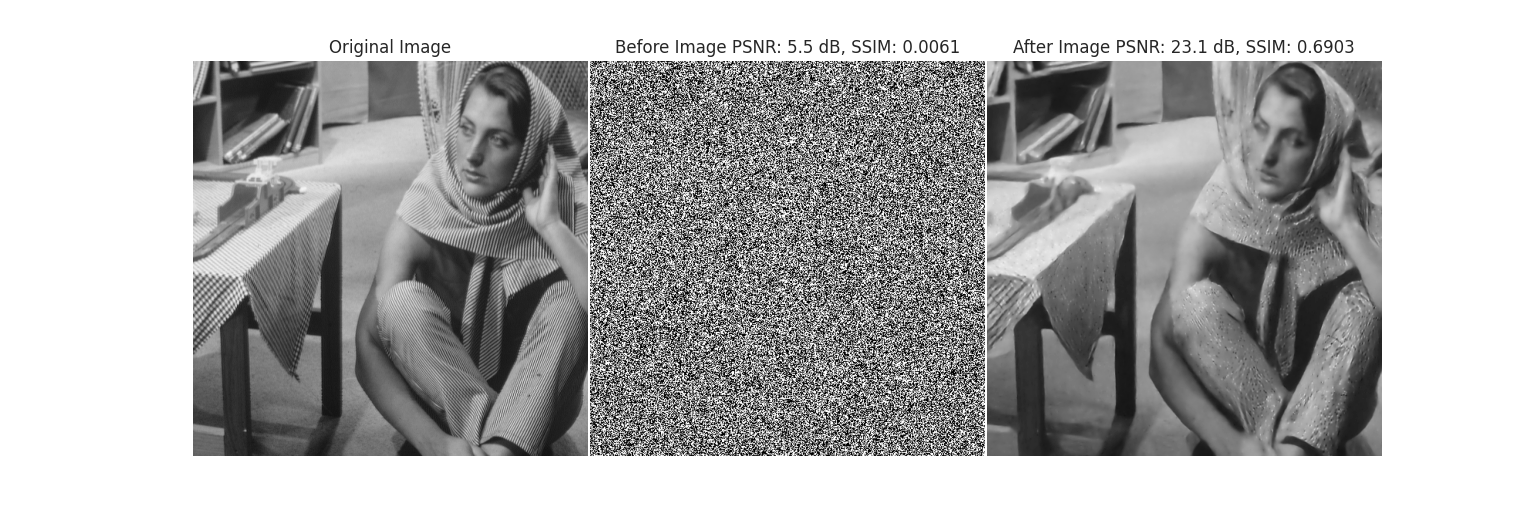
\includegraphics[width=\textwidth]{assets/240_sap_saltnet.png}
        \caption{SaltNet (Salt \& Pepper, 240/250)}
    \end{subfigure}
    \hfill
    \begin{subfigure}{0.48\textwidth}
        \centering
        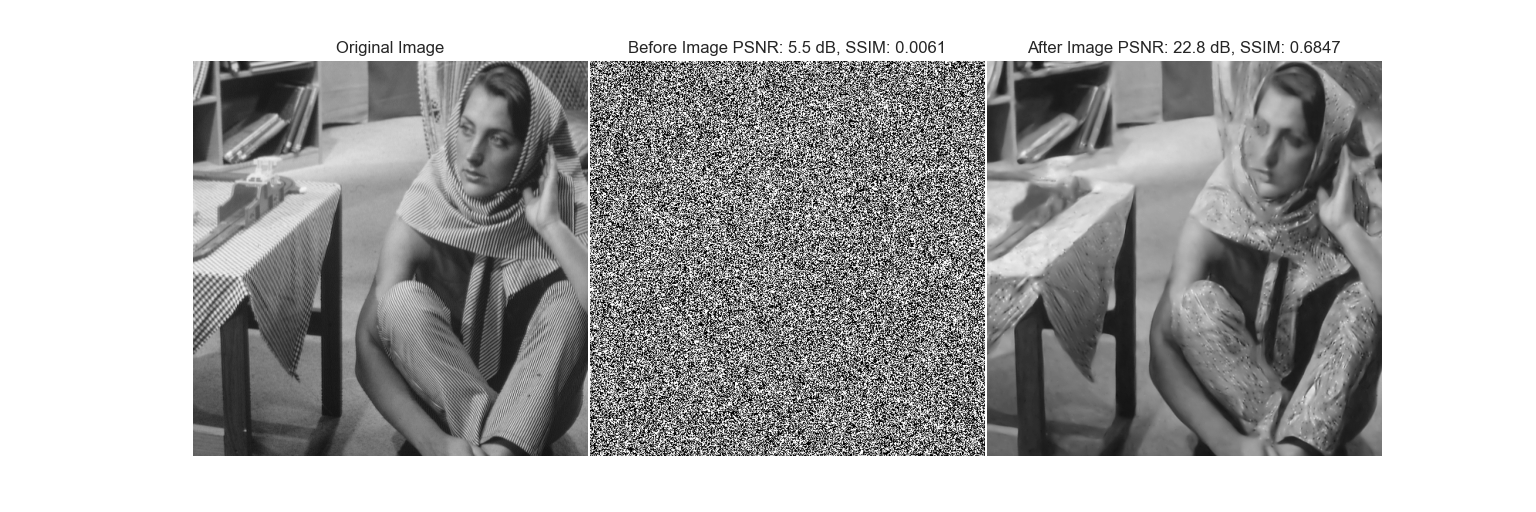
\includegraphics[width=\textwidth]{assets/240_sap_restormer.png}
        \caption{Restormer (Salt \& Pepper, 240/250)}
    \end{subfigure}
    \begin{subfigure}{0.48\textwidth}
        \centering
        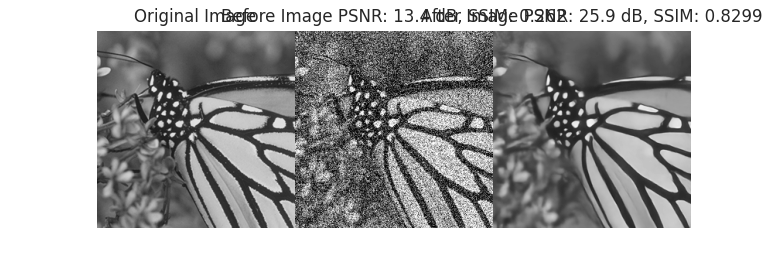
\includegraphics[width=\textwidth]{assets/60_gau_2_saltnet.png}
        \caption{SaltNet (Gaussian, 60/250)}
    \end{subfigure}
    \hfill
    \begin{subfigure}{0.48\textwidth}
        \centering
        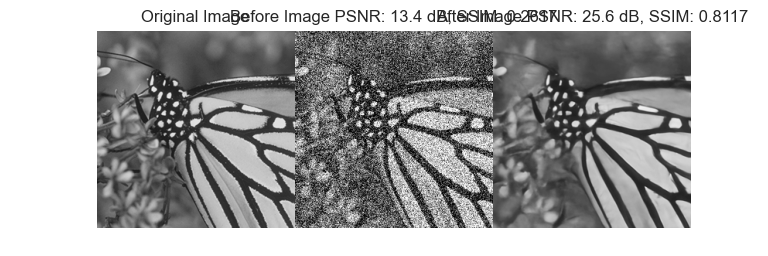
\includegraphics[width=\textwidth]{assets/60_gau_2_restormer.png}
        \caption{Restormer (Gaussian, 60/250)}
    \end{subfigure}
    \begin{subfigure}{0.48\textwidth}
        \centering
        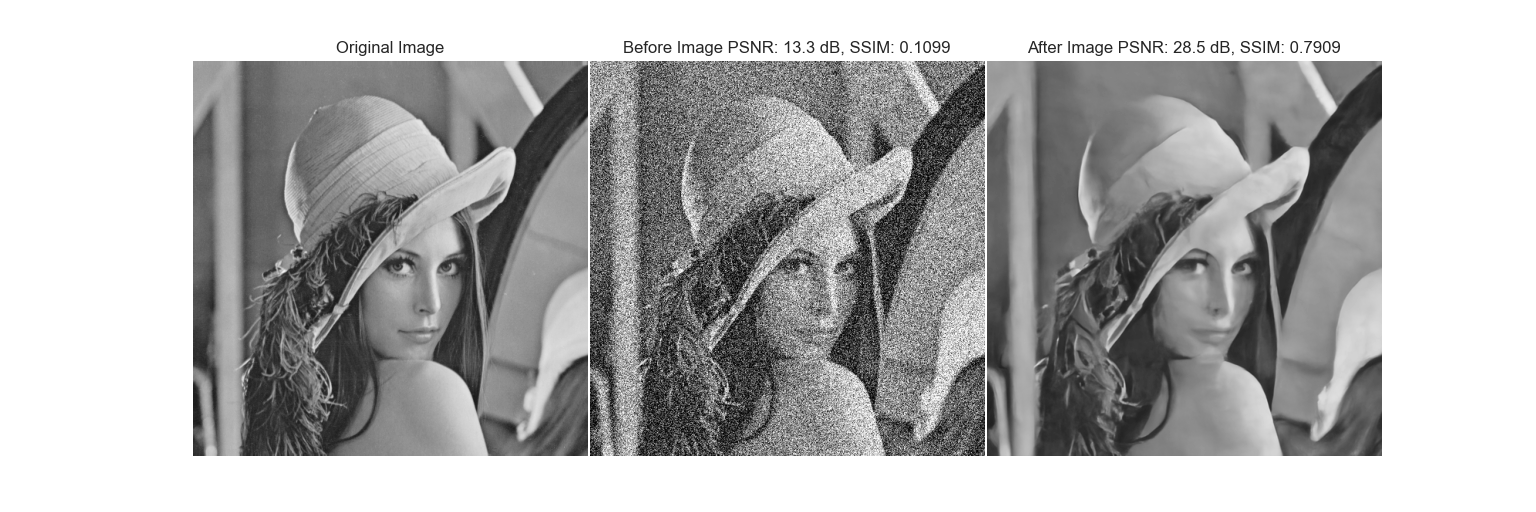
\includegraphics[width=\textwidth]{assets/60_gau_saltnet.png}
        \caption{SaltNet (Gaussian, 60/250)}
    \end{subfigure}
    \hfill
    \begin{subfigure}{0.48\textwidth}
        \centering
        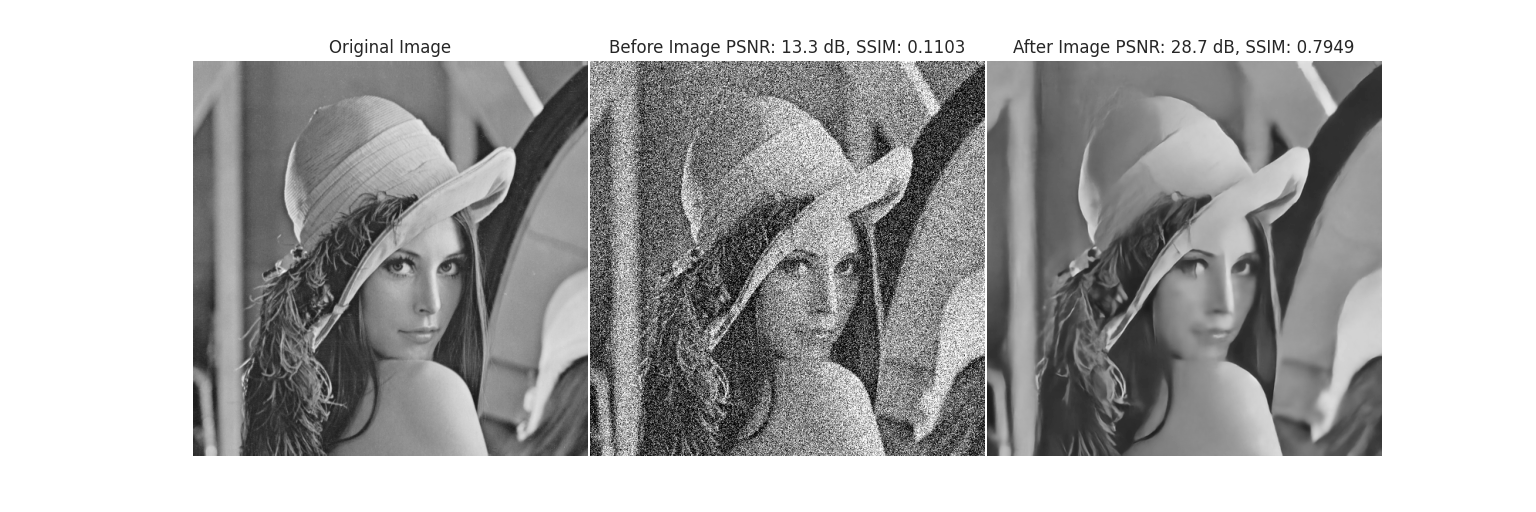
\includegraphics[width=\textwidth]{assets/60_gau_restormer.png}
        \caption{Restormer (Gaussian, 60/250)}
    \end{subfigure}
    \begin{subfigure}{0.48\textwidth}
        \centering
        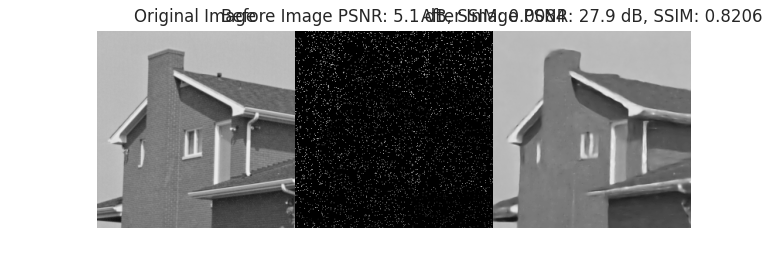
\includegraphics[width=\textwidth]{assets/240_bern_saltnet.png}
        \caption{SaltNet (Bernoulli, 240/250)}
    \end{subfigure}
    \hfill
    \begin{subfigure}{0.48\textwidth}
        \centering
        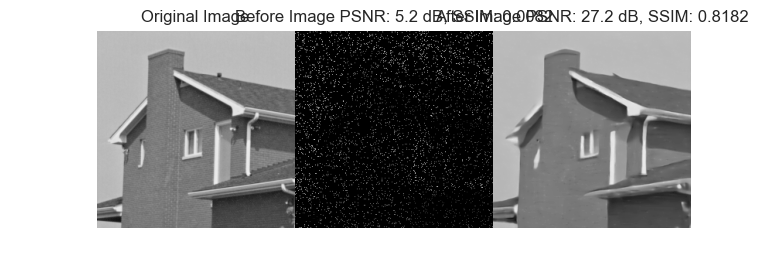
\includegraphics[width=\textwidth]{assets/240_bern_restormer.png}
        \caption{Restormer (Bernoulli, 240/250)}
    \end{subfigure}
    \begin{subfigure}{0.48\textwidth}
        \centering
        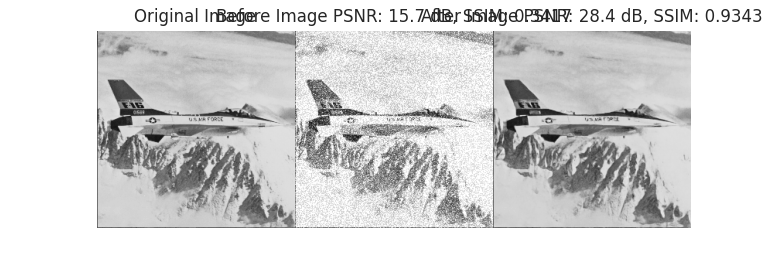
\includegraphics[width=\textwidth]{assets/240_pois_saltnet.png}
        \caption{SaltNet (Poisson, 240/250)}
    \end{subfigure}
    \hfill
    \begin{subfigure}{0.48\textwidth}
        \centering
        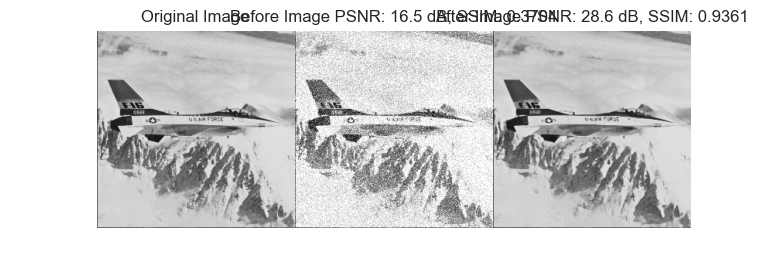
\includegraphics[width=\textwidth]{assets/240_pois_restormer.png}
        \caption{Restormer (Poisson, 240/250)}
    \end{subfigure}
    % \begin{subfigure}{0.48\textwidth}
    %     \centering
    %     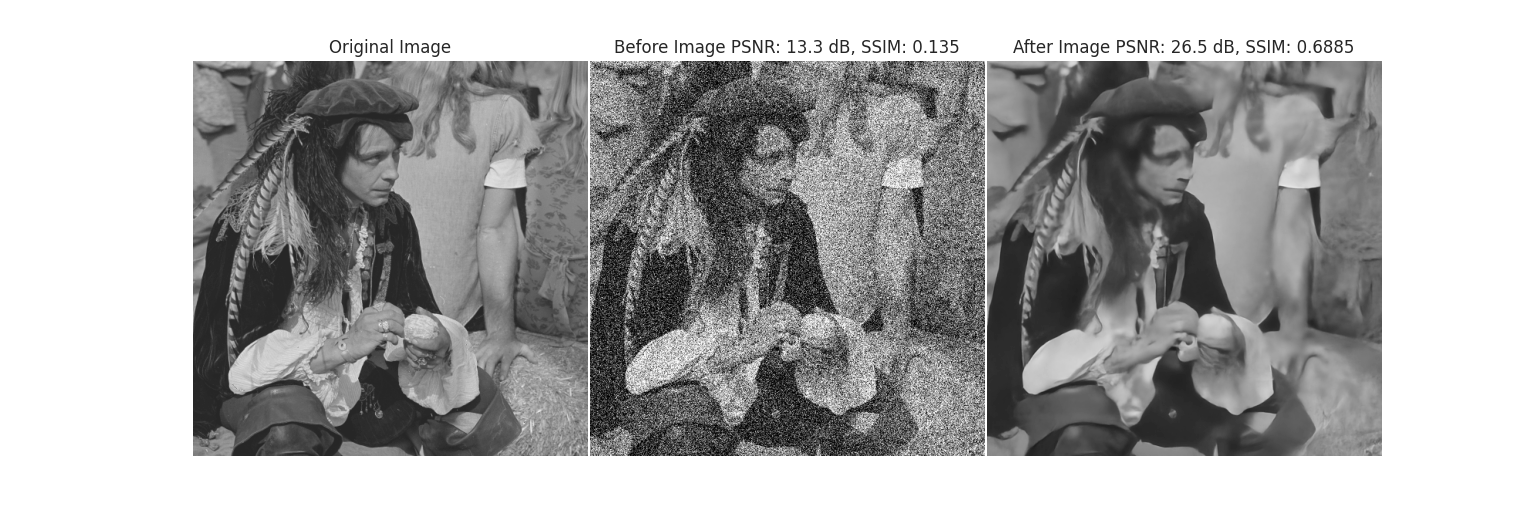
\includegraphics[width=\textwidth]{assets/60_gau_3_saltnet.png}
    %     \caption{SaltNet (Gaussian, 60/250)}
    % \end{subfigure}
    % \hfill
    % \begin{subfigure}{0.48\textwidth}
    %     \centering
    %     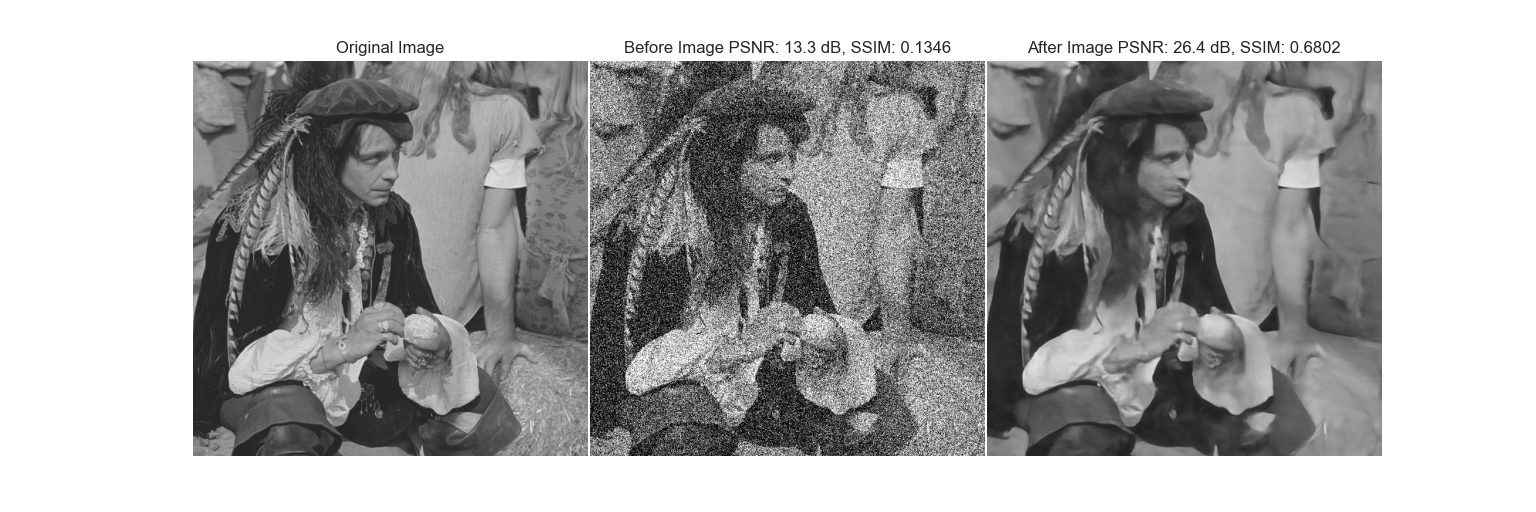
\includegraphics[width=\textwidth]{assets/60_gau_3_restormer.png}
    %     \caption{Restormer (Gaussian, 60/250)}
    % \end{subfigure}
    % \begin{subfigure}{0.48\textwidth}
    %     \centering
    %     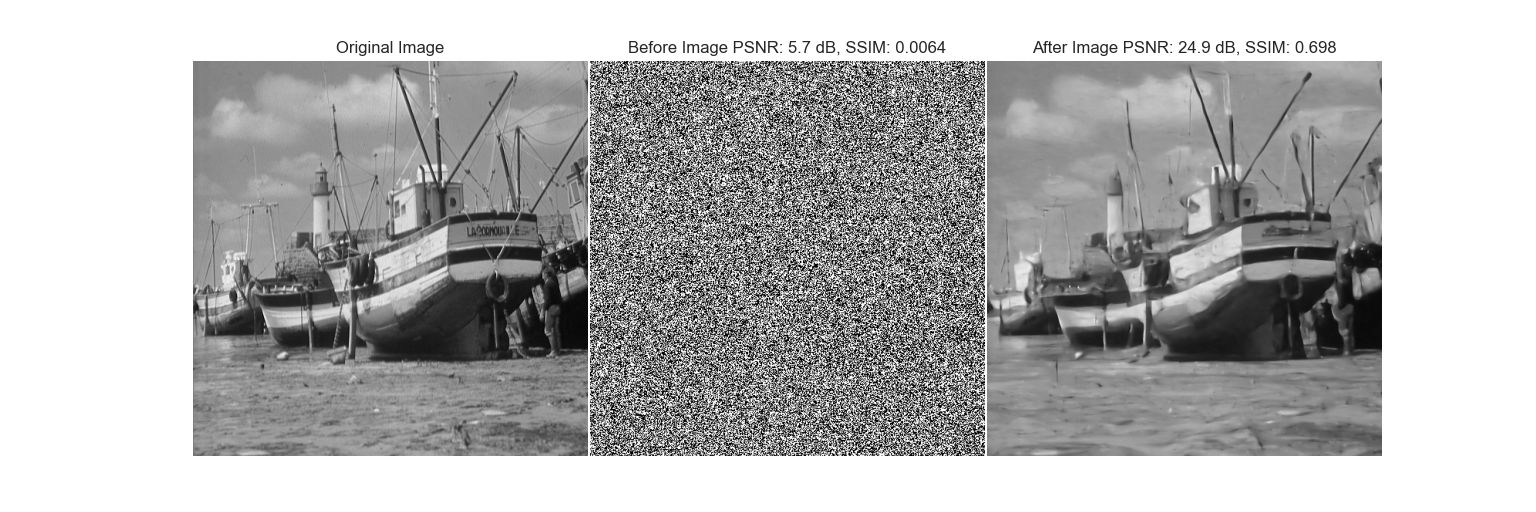
\includegraphics[width=\textwidth]{assets/240_sap_2_restormer.png}
    %     \caption{SaltNet (Salt \& Pepper, 240/250)}
    % \end{subfigure}
    % \hfill
    % \begin{subfigure}{0.48\textwidth}
    %     \centering
    %     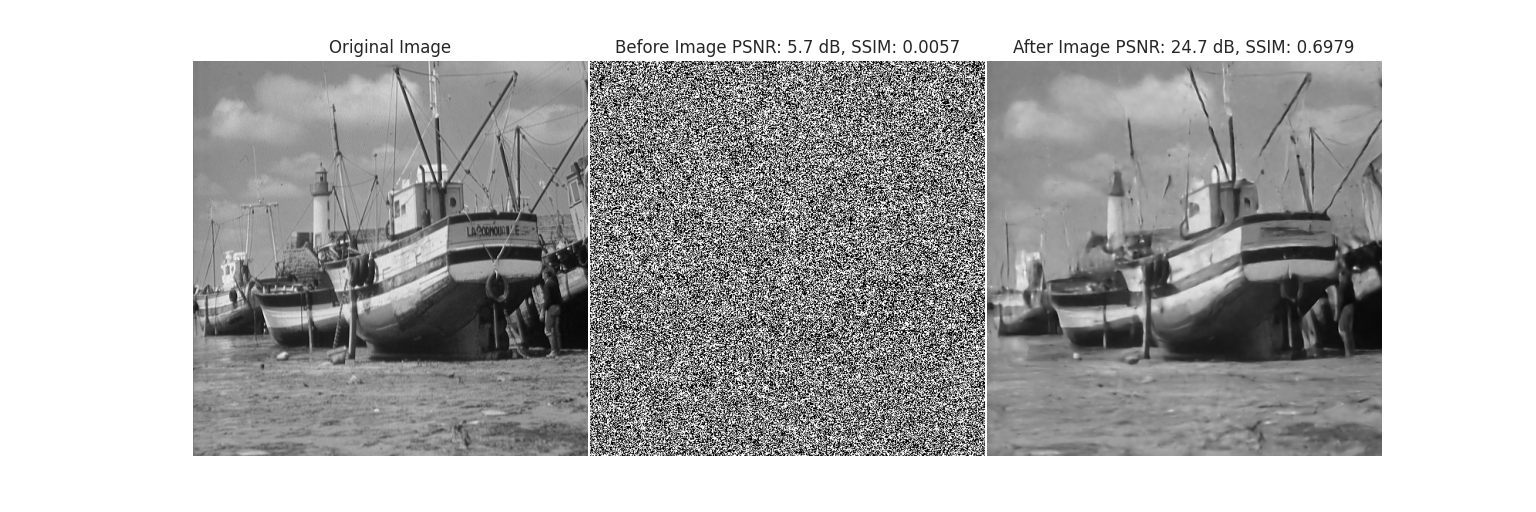
\includegraphics[width=\textwidth]{assets/240_sap_2_saltnet.png}
    %     \caption{Restormer (Salt \& Pepper, 240/250)}
    % \end{subfigure}
    % \caption{Qualitative Results}
\end{figure}

\pagebreak

\subsection{Performance Comparisons}

SaltNet is shown through the results below to be much more resource efficient than Restormer.

\begin{table}[!hbt]
    \centering
    \caption{Performance Comparison}
    \begin{tabular}{lcccccc}
    \toprule
    Size & Restormer Mem. & Our Model Mem. & Restormer Thr. & Our Model Thr. \\
    (px) & (bytes) & (bytes) & (im/s) & (im/s) \\
    \midrule
    64 & 2.60E+08 & 2.23E+08 & 25.15 & 45.27 \\
    128 & 3.22E+08 & 1.43E+08 & 24.12 & 43.95 \\
    256 & 5.45E+08 & 3.22E+08 & 21.42 & 41.60 \\
    512 & 1.77E+09 & 1.04E+09 & 6.36 & 31.63 \\
    1024 & 6.74E+09 & 3.90E+09 & 1.22 & 23.61 \\
    2048 & 1.53E+10 & OOM & OOM & 2.52 \\
    4096 & OOM & OOM & OOM & OOM \\
    \bottomrule
    \end{tabular}
\end{table}

\begin{figure}[!hbt]
        \centering
        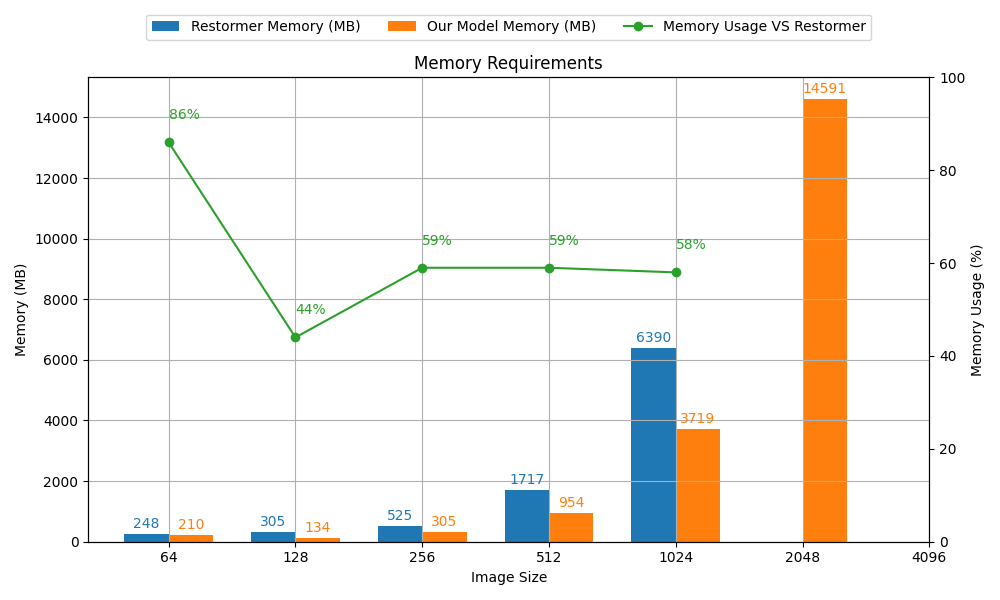
\includegraphics[width=\textwidth]{assets/memory-requirements.png}
        \caption{SaltNet (Poisson, 240/250)}
\end{figure}
\begin{figure}[!hbt]
        \centering
        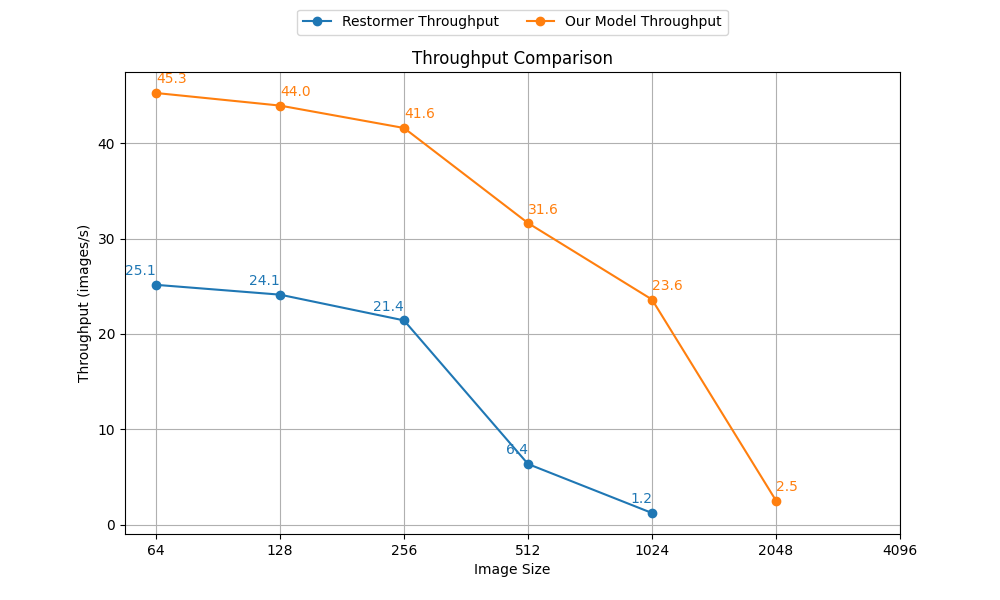
\includegraphics[width=\textwidth]{assets/throughput.png}
        \caption{Restormer (Poisson, 240/250)}
\end{figure}

\section{Ablation Study}
\label{sec:ablation_study}
    To dissect the contribution of individual components to SaltNet's overall performance, we conducted an ablation study by systematically removing or reducing key architectural elements.  This analysis allows us to quantify the importance of each module and understand their specific roles in the denoising process.

\subsection{Ablated Model Configurations}

We evaluated the following variants of the SaltNet architecture:

\begin{itemize}
    \item \textbf{SaltNet (5 Transformer Blocks)}:  This variant reduces the number of Transformer blocks in SaltNet from 10 to 5, while keeping all other components unchanged. This aims to assess the impact of Transformer block depth on performance.
    \item \textbf{SaltNet w/o Transformer Blocks}:  This variant completely removes the Transformer block stack, evaluating the importance of global attention mechanisms in SaltNet.
    \item \textbf{SaltNet w/o Anisotropic Diffusion}: In this configuration, the Anisotropic Diffusion branch is removed entirely. This ablation investigates the contribution of the novel anisotropic diffusion blocks in handling different noise types.
    \item \textbf{SaltNet w/o SeConv}:  Here, the SeConv branch is removed, isolating the effect of the SeConv blocks, which are specifically designed for impulse noise reduction.
    \item \textbf{SaltNet w/o AutoEncoder}: In this version, the final AutoEncoder post-processing module is removed, allowing us to assess its contribution to the final denoising quality.
\end{itemize}

All other architectural parameters and training procedures remained consistent with the full SaltNet model described in the previous sections, ensuring a controlled ablation study.

The ablation study followed the same experimental methodology as described in Section \ref{sec:experimental_results}

\subsection{Quantitative Results and Analysis}

Below are the average PSNR and SSIM scores of each ablation experiment (average across all datasets)

It is possible to rank the SaltNet components in terms of highest impact on accuracy as follows:

\begin{itemize}
\item Transformer Blocks
\item U-net Module
\item Seconv Blocks
\item Anisotropic Diffusion Blocks
\end{itemize}

\begin{table}[!hbt]
    \centering
    \caption{Ablation Study Results - Gaussian Test}
    \begin{tabular}{lcccccccc}
    \toprule
     & \multicolumn{4}{c}{PSNR} & \multicolumn{4}{c}{SSIM} \\
    \cmidrule(lr){2-5} \cmidrule(lr){6-9}
     & 15 & 25 & 50 & 60 & 15 & 25 & 50 & 60 \\
    \midrule
    5 Transformers & 31.35 & 28.98 & 25.90 & 25.12 & 0.9040 & 0.8541 & 0.7543 & 0.7227 \\
    No Anisotropic I & 31.26 & 28.93 & 25.85 & 25.07 & 0.9058 & 0.8539 & 0.7532 & 0.7221 \\
    No Seconv & 30.66 & 28.35 & 25.38 & 24.62 & 0.8992 & 0.8440 & 0.7389 & 0.7063 \\
    No Transformers & 29.22 & 25.96 & 24.80 & 24.47 & 0.8377 & 0.7337 & 0.7187 & 0.6985 \\
    No Unet & 30.97 & 28.54 & 25.31 & 24.48 & 0.8924 & 0.8348 & 0.7222 & 0.6864 \\
    \underline{Baseline} & \underline{31.38} & \underline{29.08} & \underline{25.99} & \underline{25.19} & \underline{0.9057} & \underline{0.8566} & \underline{0.7560} & \underline{0.7242} \\
    \bottomrule
    \end{tabular}
\end{table}

\begin{table}[!hbt]
    \centering
    \caption{Ablation Study Results - PSNR}
    \begin{tabular}{lcccccccccc}
    \toprule
    Dataset & 150 & 160 & 170 & 180 & 190 & 200 & 210 & 220 & 230 & 240 \\
    \midrule
    \textbf{BERNOULLI} \\
    5 Transform & 29.70 & 29.08 & 28.45 & 27.78 & 27.09 & 26.33 & 25.50 & 24.55 & 23.43 & 21.97 \\
    No Anisotropic Block & 29.59 & 29.00 & 28.36 & 27.71 & 27.02 & 26.27 & 25.43 & 24.49 & 23.39 & 21.94 \\
    No Seconv & 29.59 & 28.98 & 28.33 & 27.64 & 26.91 & 26.16 & 25.31 & 24.37 & 23.26 & 21.82 \\
    No Transform & 28.52 & 27.95 & 27.36 & 26.74 & 26.08 & 25.37 & 24.60 & 23.71 & 22.68 & 21.32 \\
    No Unet & 28.72 & 28.10 & 27.47 & 26.79 & 26.08 & 25.32 & 24.51 & 23.58 & 22.52 & 21.20 \\
    \underline{Baseline} & \underline{30.10} & \underline{29.48} & \underline{28.84} & \underline{28.15} & \underline{27.43} & \underline{26.64} & \underline{25.78} & \underline{24.81} & \underline{23.61} & \underline{22.06} \\
    \midrule
    \textbf{POISSON} \\
    5 Transform & 30.79 & 30.59 & 30.44 & 30.17 & 30.04 & 29.79 & 29.63 & 29.53 & 29.40 & 29.22 \\
    No Anisotropic Block & 30.82 & 30.60 & 30.46 & 30.21 & 29.98 & 29.86 & 29.63 & 29.53 & 29.39 & 29.17 \\
    No Seconv & 30.65 & 30.40 & 30.26 & 30.08 & 29.87 & 29.73 & 29.54 & 29.38 & 29.16 & 29.00 \\
    No Transform & 29.46 & 29.26 & 29.08 & 28.89 & 28.76 & 28.54 & 28.36 & 28.21 & 28.01 & 27.81 \\
    No Unet & 30.38 & 30.09 & 29.91 & 29.69 & 29.50 & 29.31 & 29.10 & 28.94 & 28.72 & 28.56 \\
    \underline{Baseline} & \underline{31.48} & \underline{31.19} & \underline{30.99} & \underline{30.83} & \underline{30.58} & \underline{30.34} & \underline{30.16} & \underline{30.00} & \underline{29.79} & \underline{29.54} \\
    \midrule
    \textbf{SAP} \\
    5 Transform & 29.24 & 28.65 & 28.03 & 27.42 & 26.75 & 26.00 & 25.17 & 24.26 & 23.16 & 21.71 \\
    No Anisotropic Block & 29.20 & 28.59 & 28.00 & 27.35 & 26.65 & 25.94 & 25.12 & 24.18 & 23.07 & 21.65 \\
    No Seconv & 28.67 & 28.20 & 27.68 & 27.05 & 26.19 & 25.42 & 24.68 & 23.76 & 22.72 & 21.32 \\
    No Transform & 27.74 & 27.21 & 26.64 & 26.03 & 25.42 & 24.74 & 24.01 & 23.19 & 22.21 & 20.88 \\
    No Unet & 28.33 & 27.73 & 27.14 & 26.49 & 25.79 & 25.04 & 24.26 & 23.35 & 22.33 & 20.99 \\
    \underline{Baseline} & \underline{29.87} & \underline{29.27} & \underline{28.64} & \underline{27.97} & \underline{27.25} & \underline{26.49} & \underline{25.62} & \underline{24.65} & \underline{23.47} & \underline{21.90} \\
    \bottomrule
    \end{tabular}
\end{table}

\begin{table}[!hbt]
    \centering
    \caption{Ablation Study Results - SSIM}
    \begin{tabular}{lcccccccccc}
    \toprule
    Noise Density & 150 & 160 & 170 & 180 & 190 & 200 & 210 & 220 & 230 & 240 \\
    \midrule
    \textbf{BERNOULLI} \\
    5 Transform & 0.926 & 0.916 & 0.904 & 0.890 & 0.873 & 0.853 & 0.826 & 0.791 & 0.740 & 0.661 \\
    No Anisotropic Block & 0.925 & 0.916 & 0.904 & 0.889 & 0.873 & 0.852 & 0.826 & 0.790 & 0.740 & 0.661 \\
    No Seconv & 0.921 & 0.909 & 0.897 & 0.882 & 0.864 & 0.842 & 0.814 & 0.778 & 0.725 & 0.645 \\
    No Transform & 0.906 & 0.894 & 0.880 & 0.864 & 0.844 & 0.820 & 0.790 & 0.751 & 0.699 & 0.619 \\
    No Unet & 0.911 & 0.899 & 0.886 & 0.869 & 0.850 & 0.826 & 0.796 & 0.757 & 0.703 & 0.623 \\
    \underline{Baseline} & \underline{0.930} & \underline{0.921} & \underline{0.909} & \underline{0.896} & \underline{0.880} & \underline{0.860} & \underline{0.835} & \underline{0.800} & \underline{0.750} & \underline{0.671} \\
    \midrule
    \textbf{POISSON} \\
    5 Transform & 0.939 & 0.936 & 0.933 & 0.929 & 0.926 & 0.921 & 0.918 & 0.916 & 0.912 & 0.908 \\
    No Anisotropic Block & 0.941 & 0.938 & 0.935 & 0.930 & 0.927 & 0.924 & 0.919 & 0.916 & 0.912 & 0.908 \\
    No Seconv & 0.941 & 0.937 & 0.935 & 0.931 & 0.927 & 0.924 & 0.919 & 0.916 & 0.912 & 0.907 \\
    No Transform & 0.920 & 0.915 & 0.911 & 0.906 & 0.901 & 0.896 & 0.890 & 0.884 & 0.878 & 0.869 \\
    No Unet & 0.935 & 0.930 & 0.927 & 0.923 & 0.919 & 0.915 & 0.911 & 0.906 & 0.902 & 0.897 \\
    \underline{Baseline} & \underline{0.949} & \underline{0.946} & \underline{0.944} & \underline{0.941} & \underline{0.937} & \underline{0.933} & \underline{0.930} & \underline{0.926} & \underline{0.923} & \underline{0.917} \\
    \midrule
    \textbf{SAP} \\
    5 Transform & 0.922 & 0.912 & 0.900 & 0.886 & 0.869 & 0.848 & 0.820 & 0.784 & 0.733 & 0.652 \\
    No Anisotropic Block & 0.923 & 0.913 & 0.901 & 0.886 & 0.869 & 0.848 & 0.821 & 0.784 & 0.733 & 0.652 \\
    No Seconv & 0.917 & 0.906 & 0.893 & 0.878 & 0.859 & 0.836 & 0.808 & 0.769 & 0.717 & 0.636 \\
    No Transform & 0.897 & 0.885 & 0.870 & 0.853 & 0.833 & 0.807 & 0.776 & 0.737 & 0.682 & 0.601 \\
    No Unet & 0.908 & 0.896 & 0.883 & 0.867 & 0.847 & 0.823 & 0.792 & 0.752 & 0.696 & 0.609 \\
    \underline{Baseline} & \underline{0.929} & \underline{0.919} & \underline{0.909} & \underline{0.895} & \underline{0.879} & \underline{0.859} & \underline{0.832} & \underline{0.797} & \underline{0.747} & \underline{0.666} \\
    \bottomrule
    \end{tabular}
\end{table}

\pagebreak

\section{Resources}
\label{sec:resources}

\begin{itemize}
\item Code: The complete SaltNet project code, including the implementation of Restormer, can be found at \url{https://github.com/mostafa-k-m/seasalt}.
\item SaltNet vs. Restormer Results: The full set of experimental results for the SaltNet vs. Restormer comparison, including all images and numerical data, can be accessed at \url{https://nileuniversity-my.sharepoint.com/:u:/g/personal/mos_kamal_nu_edu_eg/ET7VEjGbgyBCiAy7t8YxEIoB9dHZPm5WET6ajmhZCnMP4Q?e=C31VDP}.
\item Ablation Experiments Results: The complete results of the ablation experiments, with all images and numerical data, are available at \url{https://nileuniversity-my.sharepoint.com/:u:/g/personal/mos_kamal_nu_edu_eg/EWr7E1_KaRdAmpP2saWx8-MBXGOIvXEuGwPJ4rOI4Cn0ng?e=hwMfvx}.
\item Model Weights: The model weights for SaltNet, Restormer, and each of the ablation models can be downloaded from \url{https://nileuniversity-my.sharepoint.com/:u:/g/personal/mos_kamal_nu_edu_eg/EW8doN45lHNMgRMObz0Ewu0Bn4ZHBWkP47JqUGLgxh1Eag?e=2I4fyicom}.
\end{itemize}

\section*{Acknowledgements}
\label{sec:acknowledgements}
I would like to express my sincere gratitude to my professor, Dr. Walid Al-Atabany, for his invaluable guidance, patience, and understanding throughout this research project. His support and encouragement were instrumental in the successful completion of this work.

\label{sec:references}
\begin{thebibliography}{12}
    \bibitem{Rafiee2021} A. A. Rafiee and M. Farhang, "A deep convolutional neural network for salt-and-pepper noise removal using selective convolutional blocks," \textit{arXiv preprint arXiv:2104.06445}, 2021.
    \bibitem{Zamir2022} S. W. Zamir, A. Arora, S. Khan, M. Hayat, F. S. Khan, and M.-H. Yang, "Restormer: Efficient transformer for high-resolution image restoration," in \textit{Proceedings of the IEEE/CVF Conference on Computer Vision and Pattern Recognition}, 2022, pp. 1774-1784.
    \bibitem{Wu2022} J. Wu, W. Liu, C. Li, T. Jiang, I. M. Shariful, H. Sun, X. Li, X. Li, X. Huang, and M. Grzegorzek, "A State-of-the-art Survey of U-Net in Microscopic Image Analysis: from Simple Usage to Structure Modification," \textit{Unpublished manuscript}, arXiv:2202.06465, 2022.
    \bibitem{Zhang2017} K. Zhang, W. Zuo, Y. Chen, D. Meng, and L. Zhang, "Beyond a Gaussian denoiser: Residual learning of deep CNN for image denoising," \textit{IEEE Transactions on Image Processing}, vol. 26, no. 7, pp. 3142-3155, 2017.
    \bibitem{Zhang2018} K. Zhang, W. Zuo, and L. Zhang, "FFDNet: Toward a fast and flexible solution for CNN-based image denoising," \textit{IEEE Transactions on Image Processing}, vol. 27, no. 9, pp. 4608-4622, 2018.
    \bibitem{Memis2021} S. Memiş and U. Erkan, "Different adaptive modified Riesz mean filter for high-density salt-and-pepper noise removal in grayscale images," \textit{European Journal of Science and Technology}, no. 23, pp. 359-367, 2021.
    \bibitem{Zhao2017} H. Zhao, O. Gallo, I. Frosio, and J. Kautz, "Loss functions for image restoration with neural networks," \textit{IEEE Transactions on Computational Imaging}, vol. 3, no. 1, pp. 1-11, Mar. 2017.
    \bibitem{Pessoa2023} J. Pessoa, "pytorch-msssim: MS-SSIM for PyTorch," GitHub repository, 2023. Available: \url{https://github.com/jorge-pessoa/pytorch-msssim}.
    \bibitem{Martin01} D. Martin, C. Fowlkes, D. Tal, and J. Malik, "A database of human segmented natural images and its application to evaluating segmentation algorithms and measuring ecological statistics," in \textit{Proceedings of the Eighth IEEE International Conference on Computer Vision (ICCV 2001)}, vol. 2, pp. 416–423, 2001.
    \bibitem{Kodak} R. Franzen, “Kodak lossless true color image suite,” source: http://r0k.us/graphics/kodak, vol. 4, 1999.
    \bibitem{Huang2015} J. B. Huang, A. Singh, N. Ahuja, and M. H. Yang, "Single image super-resolution from transformed self-exemplars," in \textit{Proceedings of the IEEE Conference on Computer Vision and Pattern Recognition (CVPR)}, pp. 5197–5206, 2015.
    \bibitem{Set12} J. Mairal, F. Bach, J. Ponce, G. Sapiro, and A. Zisserman, “Non-local sparse models for image restoration,” in Proc. Int. Conf. Comput. Vis., 2009, pp. 2272–2279.
\end{thebibliography}
\end{document}